%!TEX program = pdflatex

\documentclass[12pt,a4paper]{report}
 
\usepackage[top=3cm, bottom=2cm, left=3cm, right=2cm,a4paper]{geometry}
\usepackage{setspace}
\usepackage{appendix}
\usepackage{verbatim}
%\singlespacing
\onehalfspacing 
%\doublespacing

\usepackage{indentfirst}

%\setlength{\parindent}{3.0cm}  % Altere o espaçamento do parágrafo aqui.

\usepackage[brazil]{babel}
\usepackage[utf8]{inputenc}
\usepackage{float}
\usepackage{graphicx,psfrag}
\newcommand\cincludegraphics[2][]{\raisebox{-0.3\height}{\includegraphics[#1]{#2}}}

\usepackage{multirow}

\usepackage{hyperref}
\hypersetup{
    colorlinks,
    citecolor=black,
    filecolor=black,
    linkcolor=black,
    urlcolor=black
}

\usepackage[T1]{fontenc}
%\usepackage{palatino}
\usepackage{amsmath, amsfonts, amssymb, amsthm}
\usepackage{xcolor}
\usepackage{url}
\usepackage{subcaption}
\usepackage{caption}
%\usepackage[all]{xy}
\usepackage[abnt-etal-list=0,abnt-etal-text=it,abnt-and-type=&,abnt-emphasize=bf,abnt-full-initials=yes,alf,bibjustif,abnt-repeated-author-omit=yes]{abntcite}

\usepackage{helvet}
\renewcommand{\familydefault}{\sfdefault}

\bibliographystyle{abntex2-alf}


\newtheorem{teorema}{Teorema}[chapter]
\newtheorem{lema}[teorema]{Lema}
\newtheorem{corolario}[teorema]{Corolário}
\newtheorem{proposicao}[teorema]{Proposi\c{c}\~ao}
\newtheorem{definicao}[teorema]{Defini\c{c}\~ao}
\theoremstyle{definition}
\newtheorem{exemplo}{Exemplo}
%\theoremstyle{remark}
\newtheorem*{obs}{Observação}

\newcommand{\R}{\mathbb{R}}
\newcommand{\Z}{\mathbb{Z}}
\newcommand{\F}{\mathbb{F}}
\newcommand{\I}{\mathbb{I}}
\newcommand{\LL}{\mathbb{L}}
\newcommand{\M}{\mathbb{M}}
\newcommand{\G}{\mathbb{G}}
\newcommand{\X}{\mathbf{X}}
\newcommand{\Y}{\mathbf{Y}}
\newcommand{\PX}{\mathcal{P}\left(\mathbf{X}\right)}
\newcommand{\FX}{\mathcal{F}\left(\X\right)}

\newcommand{\bb}{\begin{equation}}
\newcommand{\ee}{\end{equation}}
\newcommand{\bbb}{\begin{eqnarray}}
\newcommand{\eee}{\end{eqnarray}}
\newcommand{\benu}{\begin{enumerate}}
\newcommand{\eenu}{\end{enumerate}}
\newcommand{\tr}{\mbox{tr}}
\newcommand{\cao}{\c{c}\~ao }
\newcommand{\coes}{\c{c}\~oes }

\newcommand{\vetx}{\mathbf{x}}
\newcommand{\vety}{\mathbf{y}}
\newcommand{\vetw}{\mathbf{w}}
\newcommand{\vetn}{\mathbf{n}}
\newcommand{\ima}{\mathbf{a}}
\newcommand{\ims}{\mathbf{s}}
\newcommand{\imb}{\mathbf{b}}
\newcommand{\imt}{\mathbf{t}}

\newcommand{\alphav}{\mbox{\boldmath$\alpha$}}
\newcommand{\betav}{\mbox{\boldmath$\beta$}}
\newcommand{\thetav}{\mbox{\boldmath$\theta$}}
\newcommand{\lambdav}{\mbox{\boldmath$\lambda$}}
\newcommand{\gammav}{\mbox{\boldmath$\gamma$}}
\newcommand{\varthetav}{\mbox{\boldmath$\vartheta$}}
\newcommand{\nuv}{\mbox{\boldmath$\nu$}}
\newcommand{\sigmav}{\mbox{\boldmath$\sigma$}}

\newcommand{\tn}{\,\mathrm{t}\,}
\newcommand{\sn}{\,\mathrm{s}\,}
\newcommand{\agg}{\,\mathrm{a}\,}
\newcommand{\cc}{\, \mathtt{c} \,}
\newcommand{\bpm}{\begin{bmatrix}}
\newcommand{\epm}{\end{bmatrix}}

% \renewcommand{\rmdefault}{phv} % Arial
% \renewcommand{\sfdefault}{phv} % Arial

\usepackage[toctitles]{titlesec}
\titleformat{\chapter}
  {\normalfont\bfseries}{\thechapter}{1em}{\uppercase}
\titleformat{\section}
  {\normalfont\bfseries}{\thesection}{0.7em}{\sc}
\titleformat{\subsection}
  {\normalfont\bfseries}{\thesubsection}{0.4em}{ }


\newcommand{\capitulo}[1]{\chapter{\MakeUppercase{#1}}}
\newcommand{\secao}[1]{\section{\bf #1}}
\newcommand{\subsecao}[1]{\subsection{\bf #1}}

\titlespacing{\chapter}{0cm}{1cm}{1cm}

\usepackage{fancyhdr}
\pagestyle{fancy}
\lhead{}
\chead{}
\rhead{\thepage}
\lfoot{}
\cfoot{}
\rfoot{}
\renewcommand{\headrulewidth}{0pt}

\usepackage{tocloft}
\renewcommand{\cftpartleader}{\cftdotfill{\cftdotsep}} % for parts
\renewcommand{\cftchapleader}{\cftdotfill{\cftdotsep}} % for chapters
\renewcommand{\cftsecleader}{\cftdotfill{\cftdotsep}} % for sections

\makeatletter
\renewcommand\chapter{\if@openright\cleardoublepage\else\clearpage\fi
                    \thispagestyle{fancy}%
                    \global\@topnum\z@
                    \@afterindentfalse
                    \secdef\@chapter\@schapter}
\makeatother

\renewcommand{\chaptermark}[1]{%
\markboth{\thechapter.\ #1}{}}
\setlength{\headheight}{15pt}

\addto\captionsbrazil{\renewcommand{\contentsname}{}}
\addto\captionsbrazil{\renewcommand{\listfigurename}{}}
\addto\captionsbrazil{\renewcommand{\listtablename}{}}
\addto\captionsbrazil{\renewcommand{\bibname}{}} %inclui as configurações

% Escolhe a cor do tema do documento
\newcommand\CorTema{purple}

% insert the version .tex file
%% Automatically defined version by generate_version.js script

\newcommand\Revisao{local}

% Add if conditional, for put answears of the questions
\newif\ifanswers
\answerstrue % comment out to hide answers

\begin{document}

%
% CAPA
%
\thispagestyle{empty}

\begin{center}
    
\includegraphics[scale=0.7]{fig/logo.png}

    \vspace{.7cm}

    {\Large \uppercase{Pablo Jean Rozario}}

    \vspace{3cm}

    \Large \MakeUppercase{\textbf{PLANO DE AULA \\
            Microcontroladores - Turma 1 }}

    \vspace{3cm}

    \normalsize

    \begin{itemize}
        \item \textbf{Aula} : 2
        \item \textbf{Turma} : 1
        \item \textbf{Duração} : 4 Horas
        \item \textbf{Tema} : Inteiros e IOs
    \end{itemize}

    \vspace{3cm}

    Cambé - PR \\ \textit{Dezembro} de 2021 \\ Revisão \Revisao
\end{center}

\newpage

% Blank Page

\thispagestyle{empty}
\mbox{}
\newpage

%
% Criação dos índices.
%

\begingroup
\let\clearpage\relax
\newpage
\begin{center}
    \MakeUppercase{\bf Sumário}
\end{center}
\tableofcontents
\thispagestyle{empty}

\newpage
\begin{center}
    \MakeUppercase{\bf Lista de Figuras}
\end{center}
\listoffigures
\thispagestyle{empty}


\newpage

\chapter{Objetivos}

\section{Objetivo Geral}

Apresentar aos estudantes um pouco algumas noções de uso básicas de microcontroladores, tomando como base o STM32G0B1RE presente no kit que será utilizado durante o curso.

\section{Objetivos Específicos}

\begin{itemize}
    \item Apresentar aos estudantes os tipos de inteiro utilizados no microcontrolador;
    \item conhecer alguns registradores do microcontrolador do kit;
    \item conhecer sobre o sistema de clock do microcontrolador presente no kit;
    \item compreender o uso das entradas e saídas (IOs) do microcontrolador e como configura-las.
\end{itemize}


\chapter{Metodologia}

\section{Introdução}

Na introdução da aula, será apresentado um \textit{overview} do tema da aula, podendo utilizar os índices do sumário deste documento para enumerar os temas.

A aula será iniciada com uma pequena recapitulação dos tipos de variáveis do C, que são as seguintes:

\begin{enumerate}
    \item \textbf{char} : Tipo mais básico de dado em C. Armazena um único caractere e requer apenas um byte de memória em quase todos compiladores.
    \item \textbf{int} : Como o nome sugere, é utilizado para armazenar números inteiros.
    \item \textbf{float} : Utilizado para armazenar números decimais (numeros com valor em ponto flutuante) com precisão singular.
    \item \textbf{double} : Igual \textit{float}, mas possui precisão dupla.
\end{enumerate}

Com os tipos apresentados, utilizar o questionamento com alguns alunos escolhidos de forma aleatória, de qual o tamanho de cada tipo de variável e ir observando as resposta, sem responder se estão certos ou errados.

Com as resposta, apresentar a tabela com os respectivos tamanhos padrões das variáveis, descrito na tabela \ref{table:c_types_size}, como definido por \cite{ci:c_types}.

\begin{table}[H]
    \centering
    \caption{Tamanho padrão das variáveis em C.}
    \begin{tabular}{c|c}
    \textbf{Tipo} & \textbf{Bytes} \\ \hline
    char          & 1              \\ 
    int           & 4              \\
    float         & 4              \\ 
    double        & 8              \\ 
    \end{tabular}
    \label{table:c_types_size}
\end{table}

Após apresentado os valores padrões, mostrarei que o tamanho da variável irá DEPENDER do microcontrolador e compilador utilizados, pois cada um pode atribuir tamanhos diferentes para cada tipo de variáveis. Por exemplo, o MikroC, ao utilizar a linha PIC de 8 bits (PIC10, 12, 16 e 18), atribui tamanhos diferentes para os mesmos tipos, tais como descritos na tabela \ref{table:mikroc_sizes}, tendo como referência a própria documentação em \cite{ci:mikroc_c_types}.

\begin{table}[H]
    \centering
    \caption{Tamanho definido pelo compilador do MikroC para PIC18.}
    \begin{tabular}{c|c}
    \textbf{Type}       & \textbf{Size in bytes} \\ \hline
    (unsigned) char     & 1                      \\
    signed char         & 1                      \\
    (signed) int        & 2                      \\
    unsigned (int)      & 2                      \\
    (signed) long (int) & 4                      \\
    unsigned long (int) & 4                     
    \end{tabular}
    \label{table:mikroc_sizes}
\end{table}

O ponto é apresentar aos estudantes que, como dito pelo \textit{Dilsão}, não podemos confiar demais no compilador, e sempre que possível dizer a ele "\textit{Do This!}". Isto traz um problema grande ao operar com diferentes \textit{chipsets}.

Como exemplo, citar o uso de timestamp, e caso utilize um PIC18, o problema que isso pode causar ao portar um código de uma plataforma ARM, por exemplo.

\section{stdint.h}

Com isto, falar sobre sempre utilizar o header \textit{stdint.h} que define os tipos \textit{(u)intX\_t}, \textit{(u)int\_leastX\_t} e \textit{(u)int\_fastX\_t}, onde \textit{X} é o número de bits que a variável irá utilizar.

Dado os tipos, é importante explicar a diferença de cada tipo, sendo:

\begin{itemize}
    \item \textit{intX\_t} : Variável inteira sinalizada que ocupa o número de X bits declarados.
    \item \textit{int\_fastX\_t} : Variável inteira sem sinal que irá alocar o número de bits que implicara na melhor performance do \textit{chipset}, desde que contemple o tamanho solicitado.
    \item \textit{int\_leastX\_t} : Variável sinalizada que ocupará o menor número de bits possível que tenha pelo menos X bits.
\end{itemize}

Para auxiliar na fixação destas informações, que são mais complexas, citar exemplos. Por exemplo, em um STM32 de 32bits, variáveis uint8\_t ocuparão 1byte, uint16\_t ocupará 16bytes. No caso de variáveis uint\_fast8\_t, uint\_fast16\_t e uint\_fast32\_t ocuparão 4 bytes, pois este é o tamanho de variável que necessitará de menos instruções para executar, tem relação em geral com o alinhamento de memória do \textit{chipset}. Para mais informações pode ser consultada o \cite{ci:diff_uint}.

\textbf{Dica Didática:} No caso específico o uint\_leastX\_t operará igual ao o uintX\_t. Mas é interessante citar um \textit{chipset} "exótico" de 10 bits, apenas para facilitar o entendimento.

\section{IOs de Uso Geral (General Porpouse Inputs-Outputs)}

As portas de entradas e saídas de uso geral (GPIOs) são terminais digitais utilizados pelo microcontrolador para interagir com o mundo externo, que podem assumir função de entrada ou saída, sendo utilizados durante o \textit{runtime} do microcontrolador.

As entradas e saídas são em geral multiplexadas com funções especiais, ou seja, podem assumir outras funções que estão relacionadas aos periféricos.

Mas antes de discorrer sobre as GPIOs, é importante explicar alguns termos que são Alta Impedância (High Impedance, \textit{Hi-Z}), flutuante (\textit{Floating pin}) e o que são os resistores de \textit{Pull-Up} e \textit{Pull-Down}, descritos por \cite{ci:od_vs_pp}.

\begin{itemize}
    \item \textbf{Hi-Z} : Um terminal caracterizado por ter uma alta impedância que, de forma efetiva, mitiga uma influência no circuito externo. Utilizar como exemplo um voltímetro, que mede a tensão de um circuito sem causar influência no circuito que está sendo mensurado.
    \item \textbf{Floating pin} : Um terminal que é deixado desconectado tanto externamente quanto internamente, seu nível de tensão e lógico é indefinido e imprevisível. Nota: um terminal \textbf{Hi-Z} sem resistores de pull-up/down é dito que está flutuando (\textit{floating}).
    \item \textbf{Pull-Up/Pull-Down} : Resistores utilizados para definir um nível lógico em um terminal flutuante, um resistor de \textit{pull-up} é conectado ao barramento de alimentação e define o nível lógico 1 no terminal de entrada, enquanto que um resistor de \textit{pull-down} é conectado ao referencial (\textit{ground}) e define o nível lógico 0.
\end{itemize}

Na figura \ref{fig:basic_gpio_structure} é exibido a estrutura básica de uma GPIO do microcontrolador presente no kit utilizado.

\begin{figure}[H]
    \centering
    \caption{Estrutura básica de uma GPIO do STM32G0B1.}
    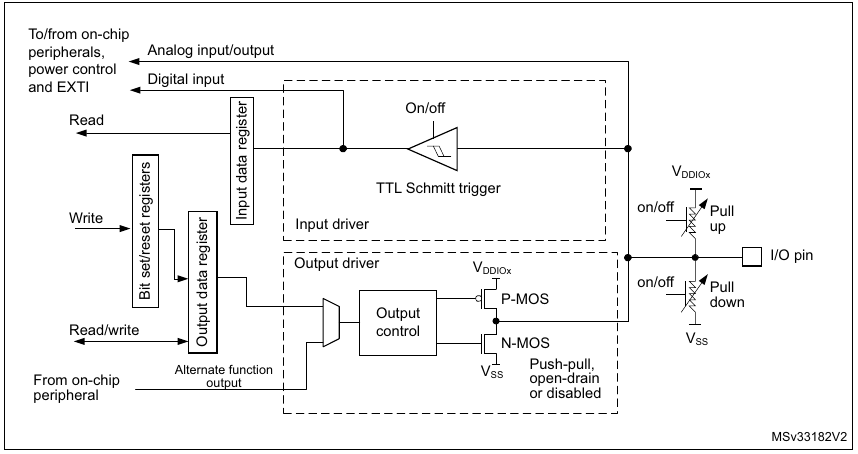
\includegraphics[scale=0.5]{fig/basic_gpio_structure.png}
    \caption*{Fonte: \cite{ci:rm0444}.}
    \label{fig:basic_gpio_structure}
\end{figure}

Para facilitar o entendimento, poderá apresentar as figuras em \ref{fig:basic_gpio_structure_faded}, onde é destacado apenas a parte de interesse, da parte de input e output, respectivamente.

\begin{figure}[H]
    \centering
    \caption{Estrutura básica de uma GPIO do STM32G0B1 com entrada e saída destacados.}
    \begin{subfigure}{0.4\textwidth}
        \centering
        \caption{Estrutura de uma entrada de uma gpio.}
        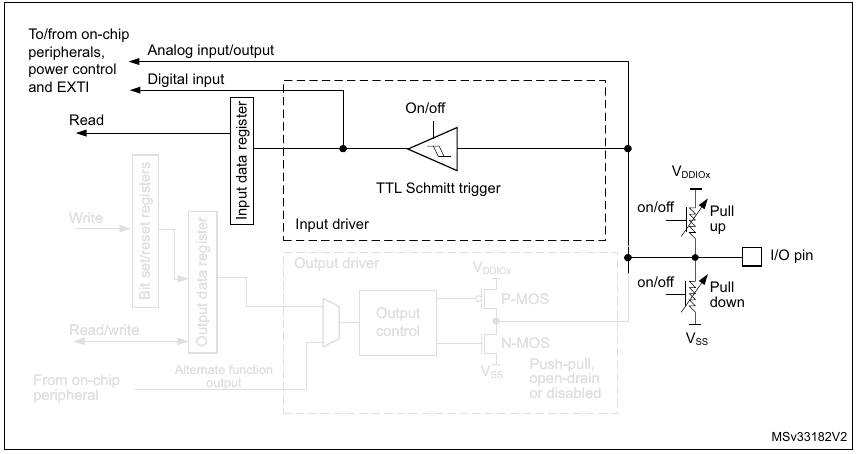
\includegraphics[width=1\linewidth]{fig/basic_gpio_structure_in.png}
    \end{subfigure}
    \begin{subfigure}{0.4\textwidth}
        \centering
        \caption{Estrutura de uma saída de uma gpio.}
        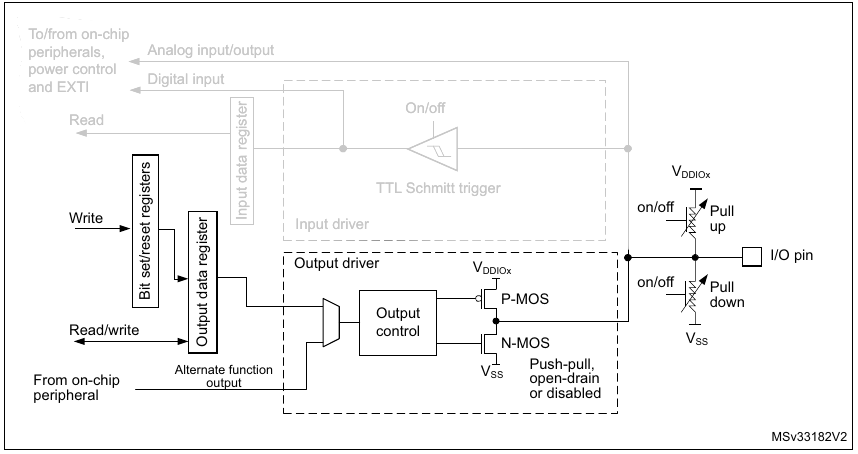
\includegraphics[width=1\linewidth]{fig/basic_gpio_structure_out.png}
    \end{subfigure}
    \caption*{Fonte: Autoria própria.}
    \label{fig:basic_gpio_structure_faded}
\end{figure}

Com as figuras destacadas, é possível focar somente no que fica habilitado ao configurar a porta como entrada ou saída.

\subsection{Output}

Quando uma porta é configurada como saída, ela tem por característica controlar se o sinal deste pino terá como nível digital 0 ou 1.

Mas, o nível de tensão depende da configuração dessa saída, se esta for configurada como \textit{push-pull}, em nível lógico 0 teremos 0V, e nível lógico 1 teremos VDD, onde VDD é a alimentação do dispositivo. Na figura \ref{fig:push_pull_schematic} é ilustrado como funciona uma porta configurada como \textit{push-pull}.

\begin{figure}[H]
    \centering
    \caption{Esquemático de uma porta configurada como saída \textit{push-pull}.}
    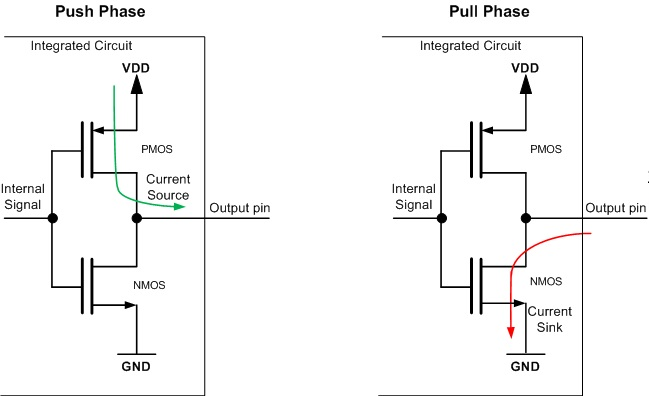
\includegraphics[scale=0.5]{fig/push_pull_schematic.jpg}
    \caption*{Fonte: Google Imagens.}
    \label{fig:push_pull_schematic}
\end{figure}

Quando uma output é configurada como \textit{open-drain} a tensão em nível lógico 0 é de 0V, mas em nível lógico 1, o sistema encontra-se em alta impedância, logo não gerando uma tensão conhecida na saída e incapacidade de fornecer corrente.

Na figura \ref{fig:open_drain_schematic} é exibido o esquemático de uma porta \textit{push-pull}.

\begin{figure}[H]
    \centering
    \caption{Esquemático de uma porta configurada como saída \textit{open-drain}.}
    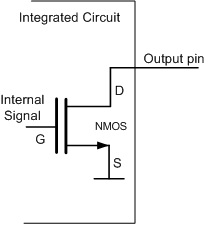
\includegraphics[scale=0.8]{fig/open_drain_schematic.jpg}
    \caption*{Fonte: Google Imagens.}
    \label{fig:open_drain_schematic}
\end{figure}

A depender do chipset que será utilizado, deve-se ler atentamente a documentação, pois alguns microcontroladores possuem portas que operam somente em \textit{open-drain}.

Em um resumo, utiliza-se muito \textit{open-drain} quando se trata de interfaces de comunicação bi-direcional (tais como I2C, OneWire), e possui maior corrente de consumo durante a transferência de energia, quando contém um resistor de pull-up.

Já o \textit{push-pull} é empregado em interfaces de comunicação unidirecionais (SPI, UART), e em geral, possui um melhor tempo de resposta se comparado ao \textit{open-drain}. Na tabela \ref{table:pp_od_signal} 

\begin{table}[H]
    \centering
    \caption{Saída de acordo com cada tipo de configuração de Output.}
    \begin{tabular}{c|c|c}
    \textbf{Sinal} & \textbf{Push Pull} & \textbf{Open Drain} \\ \hline 
    \textbf{0}     & GND                & GND                 \\ 
    \textbf{1}     & VDD                & Hi-Z               
    \end{tabular}
    \label{table:pp_od_signal}
\end{table}

\subsection{Input}

Uma porta configurada como entrada tem como finalidade realizar a leitura de uma tensão externa, neste caso de forma digital, ou seja, 0 ou 1, de acordo com o nível de tensão aplicado ao terminal. Dependendo do dispositivo que é lido pela porta de entrada é necessário utilizar os resistores de pull-up ou pull-down.

\textbf{Dica didática} : Para que haja compreensão total, utilizar como exemplo o ato de falar como uma saída (output) e o de ouvir como uma entrada (input).

Como a partir daqui iniciará os trabalhos com a implementação HAL da ST, citar e distribuir o \textit{UM2319 Description of STM32G0 HAL and low-layer drivers}, que descreve a API HAL e suas funcionalidades, descrito na referência como \cite{ci:um2319}.

\subsection{Limitações}

As GPIOs podem contem limitações que são descritas na documentação, sendo estas:

\begin{itemize}
    \item Corrente máxima do terminal: Máximo corrente que pode ser fornecida ou drenada pelo terminal (15mA para nosso kit).
    \item Corrente máxima total das IOs: Corrente máxima que pode ser drenada ou fornecida por todos os terminais (80mA para nosso kit).
\end{itemize}

\section{Configurar GPIO no STM32CubeIDE}

Para configurar uma GPIO de forma fácil no STM32CubeIDE, utilizamos o plugin do CubeMX. Primeiramente iremos iniciar um novo projeto no CubeIDE e será feita a configuração do botão e do LED pela ferramenta.

Não será informado em quais terminais que estão ligados o LED e o botão, como parte dessa primeira atividade, deverá ser consultado o documento UM2324 para obter as informações. Na figura \ref{fig:cubeIDE_project_io_1} e \ref{fig:cubeIDE_project_io_2} é possível ver como é feito a configuração de uma GPIO pelo STM32CubeIDE.

\begin{figure}[H]
    \centering
    \caption{Selecionando configuração de uma GPIO no STM32CubeIDE.}
    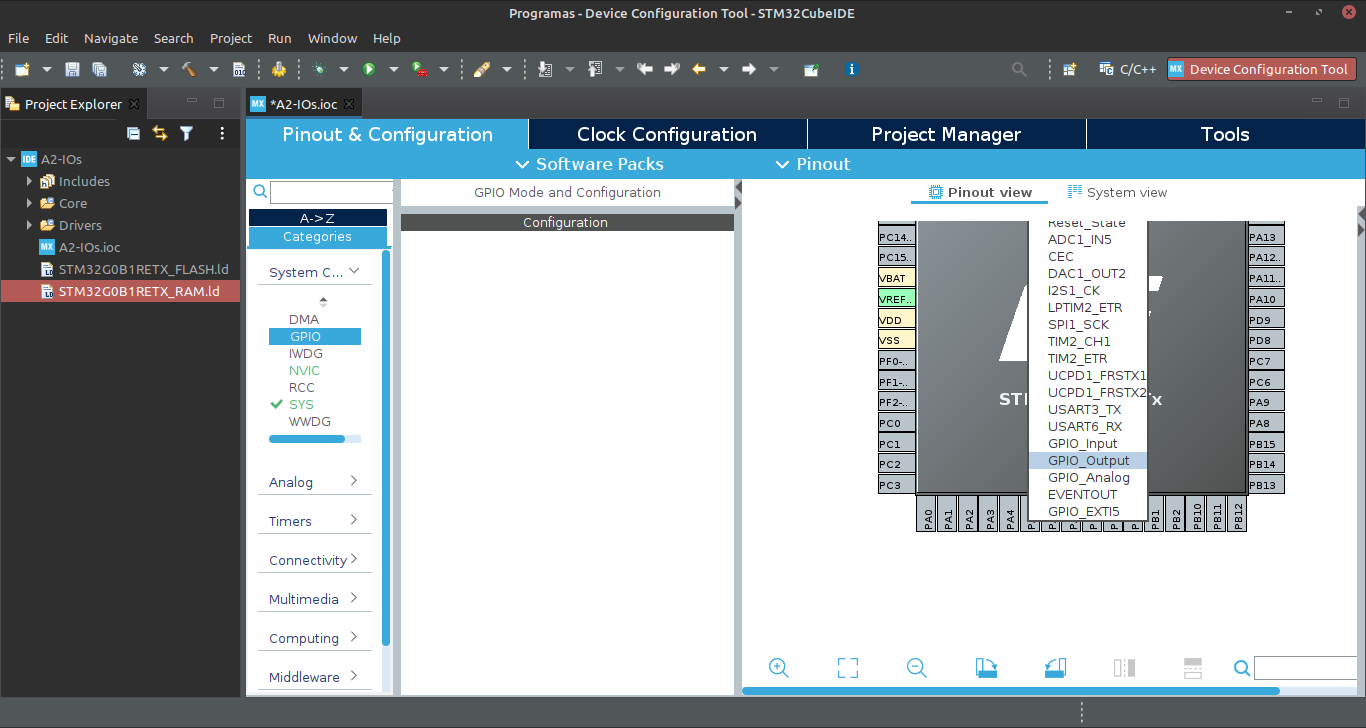
\includegraphics[scale=0.2]{fig/cubeIDE_project_io_1.png}
    \caption*{Fonte: Autoria própria.}
    \label{fig:cubeIDE_project_io_1}
\end{figure}

\begin{figure}[H]
    \centering
    \caption{Configurações de uma porta definida como saída.}
    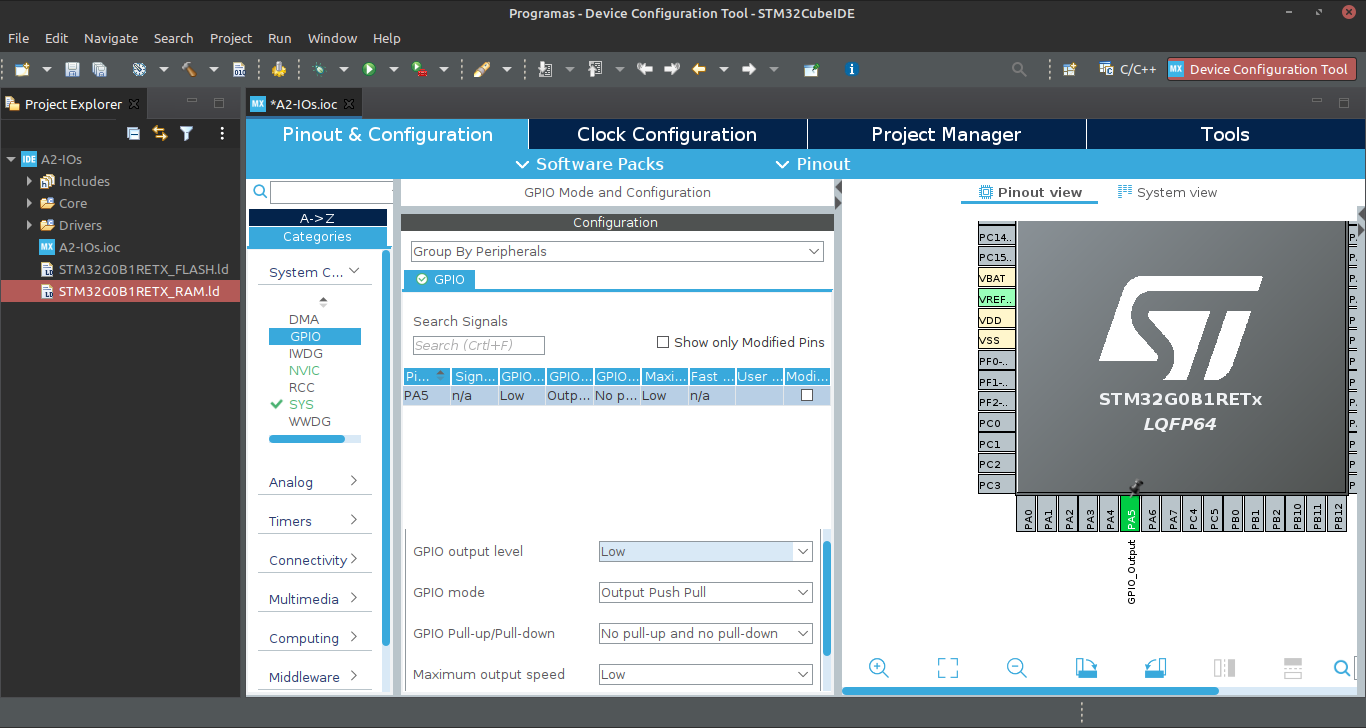
\includegraphics[scale=0.2]{fig/cubeIDE_project_io_2.png}
    \caption*{Fonte: Autoria própria.}
    \label{fig:cubeIDE_project_io_2}
\end{figure}

Comentar as duas funções importantes para trabalhar com os terminais de IO no código em C, que é a \_WritePin e \_ReadPin da biblioteca HAL. O terminal configurado pelo CubeMX tem ao seu nome atrelado dois defines, um deles para o GPIO, adicionando ao final \_GPIO\_Port, e ao número do terminal, \_Pin, temos o exemplo de uma GPIO configurada no CubeMX na figura \ref{fig:CubeMX_gpio} e chamado no código, exibido na figura \ref{fig:code_gpio_call}.

\begin{figure}[H]
    \centering
    \caption{GPIO configurada no plugin CubeMX.}
    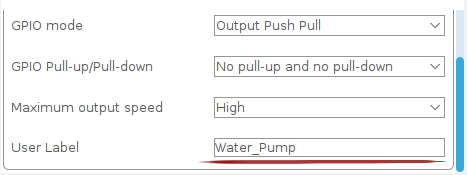
\includegraphics[scale=0.8]{fig/CubeMX_gpio.png}
    \caption*{Fonte: Autoria própria.}
    \label{fig:CubeMX_gpio}
\end{figure}

\begin{figure}[H]
    \centering
    \caption{Comando de escrita de uma GPIO para nível lógico alto.}
    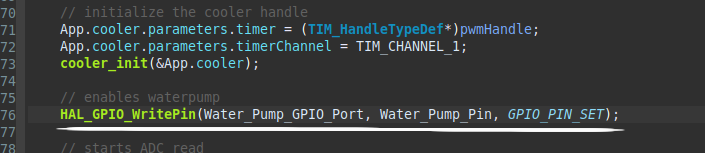
\includegraphics[scale=0.6]{fig/code_gpio_call.png}
    \caption*{Fonte: Autoria própria.}
    \label{fig:code_gpio_call}
\end{figure}

Como primeiro programa que será feito junto, apenas um exemplo para coletar a leitura do valor do botão, e um \textit{toggle} do LED LD4.

Após isto, tirada as duvidas referentes a aula, iniciar atividades referentes a \textbf{Lista de Exercícios} que está em anexo.

\newpage

\chapter{Recursos Didáticos}

Será utilizado lousa e canetas apropriadas, computador com os softwares necessários e projetor.

\chapter{Forma de Avaliação}

Avaliação será feita através das listas de exercícios para serem resolvidas durante as aulas ou no horário reservado.

\newpage

\chapter{Histórico de Revisão}

\subsection*{Revisão 1}

Primeiro documento.

\subsection*{Revisão 2}

\begin{itemize}
    \item Novo exercício na Lista de Exercícios referente a implementação de leitura por varredura.
    \item Corrigida legenda da figura \ref{fig:code_gpio_call}.
\end{itemize}

\subsection*{Revisão 3}

\begin{itemize}
    \item Removido exercícios da Lista de Exercícios.
\end{itemize}

\newpage

\begin{appendices}

    \chapter{Anexos}

    \section{Lista de Exercícios - Resolvida}
    % Macros auxiliares

\newcounter{idx}
\setcounter{idx}{1}

\newcommand{\question}[1]{ 

    \textbf{\theidx : }#1
    \stepcounter{idx}
}

\newcommand{\answer}[1]{

    \ifanswers
    {
        %\newline
        \scriptsize\color{purple}\textbf{R:} #1
    }
    \else
    \vspace{1cm}
    \fi 
}

% Cabeçalho para a Lista de Exercícios
\begin{tabular}{l|ll}
    \multirow{3}{*}{
\includegraphics[width=84px]{fig/logo.png}} & { } & {\LARGE \textbf{Lista de Exercícios \#2 }} \\
    & { } & {\Large Pado Labs - Microcontroladores} \\
    & { } & {Registradores e IOs}   
    \end{tabular}
    
    \vspace{0.5cm}
    \textit{Tips and Tricks} : Utilizar os documentos do kit para resolver os exercícios.

    \textit{Requirements} : Resolva pelo menos 7 exercícios. Exercícios com a \textit{tag} {\color{red}\textbf{Challenge}} valem por dois.
    
    \textit{Requirements} : Exercícios que requerem desenvolvimento de um código deve ser separado e zipado, com título do projeto e nome do arquivo fácil de identificar como \textit{Lista2-Ex2.rar}, \textit{L2-E2.rar}.
    \vspace{0.5cm}

    \question{Qual a vantagem de se trabalhar com os tipos da biblioteca \textit{stdint.h}}

    \answer{Permite dizer ao compilador como quer tratar as variáveis inteiras, se será o menor tamanho possível ou para oferever melhor performance, tendo controle do tamanho da variável, independente do chipset utilizado.}


    \question{Qual a principal característica de uma viariável do tipo \textit{int\_fastX\_t}?}

    \answer{Este tipo de viariável utiliza o tamanho que proverá a melhor performance possível, a depende da arquitetura.}


    \question{No nosso kit NUCLEO-G0B1RE, qual o tamanho da variável, em bytes, do int\_fast8\_t, int\_fast16\_t, int\_fast32\_t e int\_fast64\_t.}

    \answer{4, 4, 4 e 8 bytes.}


    \question{Qual a função dos registradores:
    
    \begin{itemize}
       \item GPIOx\_MODER
       \item GPIOx\_OTYPER
       \item GPIOx\_OSPEEDR
       \item GPIOx\_PUPDR
       \item GPIOx\_IDR
       \item GPIOx\_ODR
       \item GPIOx\_AFRL
    \end{itemize}}

    \answer{Seleciona o modo do GPIO, configura o tipo de saída, configura a velocidade de saída, habilita/desabilita os resistores pull-up ou pull-down, ler o valor da entrada do gpio, define o valor de saida do GPIO}


    \question{Como posso fazer para ler diretamente o registrador sem utilizar a implementação da ST? (\textit{tip}: lembre-se dos ponteiros!)}

    \answer{Declarar um ponteiro do tipo \textit{uint32\_t} e atribua a ele o endereço do registrador. Após isto, leia o conteúdo do ponteiro.}


    \question{Desenvolva um firmware que pisque o LD4 com uma frequência de 1Hz (500ms aceso, 500ms apagado)}

    \answer{\textit{Programar!}}


    \question{Desenvolva um firmware que pisque o LD4 com uma frequência de 100Hz.}

    \answer{\textit{Programar!}}


    \question{Faça um programa que pisque o LD4 em 20Hz enquanto o botão USER é pressionado e pisque com frequêcia de 5Hz ao ser solto.}

    \answer{\textit{Programar!}}


    \question{Faça a leitura dos \textit{switches} do tipo DIP de 4 posições utilizando os resistores de \textit{pull-up} ou \textit{pull-down} internos. Armazene em uma variável o valor correspondente, onde a chave 1 corresponde ao bit 0, e o bit 4 corresponde ao bit 3.}

    \answer{\textit{Programar!}}


    \question{Aproveite o exercício anterior, monte 4 LEDs e associe cada um deles a uma chave do DIP switch de 4 posições, quando a chave estiver em ON, acenda o LED, e em OFF, apague o LED.}

    \answer{\textit{Programar!}}


    \question{{\color{red}\textbf{Challenge}:} Aproveite o exercício anterior novamente, mas sem os LEDs, e exiba em um display de 7 segmentos o valor correspondente em hexadecimal (0 à F).}

    \answer{\textit{Programar!}}


    \question{{\color{red}\textbf{Challenge}:} Existe uma técnica comumente chamada de \textit{Varredura}, esta técnica consiste em ligar elemento em matriz para otimizar o uso de GPIOs, muito utilizada para acionar LEDs e realizar a leitura de botões e \textit{keypads}. Nisto, como desafio, deve-se montar o circuito da figura \ref{fig:matrix_btn_4x4} e desenvolver um firmware que faça a leitura dessas teclas e armazene em uma variável a linha e coluna da tecla pressionada (a linha e coluna deve ser numerada de 1 a 4, quando nenhuma tecla estiver pressionada, deve ser exibido o valor 0).}

    \begin{figure}[H]
        \centering
        \caption{Esquemático de uma matriz de botões 4x4.}
        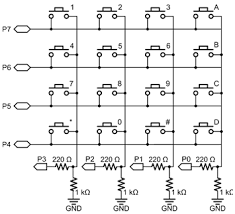
\includegraphics[scale=0.8]{fig/matrix_btn_4x4.png}
        \label{fig:matrix_btn_4x4}
    \end{figure}

    \answer{\textit{Programar!}}

  
    % ---- END OF FILE ----

\end{appendices}

\newpage

\begin{center}
    \chapter*{REFERÊNCIAS}
\end{center}


\bibliography{referencia}

\endgroup

\end{document}